\chapter{Strain-induced vector potentials: Lattice-corrections and engineered pseudo magnetic fields\label{chap:PVP}}

At the intersection of graphene's outstanding mechanical and electrical properties lies a peculiar and provocative coupling.
Certain strain distributions in graphene can trick the electrons into acting as if they were in a magnetic field.
This comes about because strain shifts the crystal momentum of the Dirac points much like the the canonical momentum is shifted in the presence of a magnetic field.
This exotic coupling is made more appealing by the two dimensional elastic nature of graphene.
Not only does the coupling exist in theory, but the material also allows the physical realization of it.

A dazzling glimpse of the feasibility and potential of strain-engineered graphene \cite{Pereira2009a,Guinea2009} has recently emerged with experiments reporting that certain strain profiles can induce Landau quantization and effective pseudomagnetic fields in excess of 300 T\cite{Levy2010,Yan2012,Yeh2011}.
Such physics strongly encourages the prospect of harnessing this unconventional interplay between graphene's unique electronic and impressive mechanical properties to control electronic transport in graphene devices \cite{Pereira2009a,Fogler2008}.

This chapter starts by discussing the theory of the strain-induced vector potentials with an emphasis on the lattice-corrections first introduced by Kitt et al \cite{Kitt2012,Kitt2013}.
This is followed by an examination of the importance of these lattice-corrections in different physical scenarios.
Finally, methods of strain engineering graphene devices are examined with an emphasis on the over pressured hour glass shaped microchamber.
This device cleverly takes advantage of plasmonics to enhance signals from higher pseudo magnetic field regions.

\section{Derivation of the strain induced vector potentials}

By distorting the graphene lattice, strain causes the following \cite{Pereira2009}:
(i) for any amount of strain, the Dirac points are displaced from the corners of the unstrained BZ and, furthermore, do not necessarily sit at the corners of the strained BZ;
(ii) the gapless and conical nature of the energy dispersion remains robust, except when the deformation is so strong that the two inequivalent Dirac points merge in a Lifshitz transition (but that probably requires strains of the order 20\%, where the tight-binding description is not reliable anymore);
(iii) at any finite density the Fermi line is deformed from the isotropic circle to an elliptical shape, and two Fermi velocities can be defined along the principal directions \cite{Pereira2009,Pereira2010c,Choi2010}.
All these modifications are significant and happen concurrently. 
Hence a complete description of the electronic and transport properties of strained graphene requires their combined consideration.
For example, the local shift of the Dirac point (i) can hinder or completely suppress electronic propagation across regions of different strain states \cite{Pereira2009a,Fogler2008}.
The anisotropy of the Fermi surface (iii) has direct bearing in measurable quantities such as the anisotropy in electrical resistivity\cite{Kim2009}, optical absorption \cite{Pereira2010c,Pellegrino2010}, and the Raman signature of the 2D peak \cite{Huang2010,Mohr2010a,Frank2011,Yoon2011}.

From the theoretical as well as technical point of view, the effects of strain are frequently considered independently, and one usually isolates the dominant effect for the physical observable of interest.
Referring to the same examples above, the strain-induced corrections to optical absorption arising from inter-band transitions are insensitive to the absolute position of the Dirac point in the BZ, but strongly depend on the velocity anisotropy \cite{Pereira2010c,Pellegrino2010}.
Likewise, the dominant effect across a strain barrier will be the relative position of the Fermi surfaces in the two regions (since this essentially determines the phase space available for transmission), and in a first approach the anisotropy is usually neglected \cite{Fogler2008,Pereira2009a}, since the full description would obfuscate the presentation of the problem.

When the strain-induced shift of the Dirac points (i) is considered independently of (ii) and (iii), it can be thought of as a pseudo vector potential \cite{Sasaki2005,Ando2006,Manes2007,CastroNeto2009,Vozmediano2010}.
This can be done because of the peculiar form of the strain corrections to the electronic dispersion in graphene.
Electrons in strained graphene are still governed by a Dirac equation, but one in which the strain modifications can be completely absorbed in the replacement $\bm{p} \to \bm{p}-e\bm{A}$ where $\bm{A}$ is the pseudo vector potential.
This matches the conventional minimal coupling scenario, which means that the electrons respond to the deformation-induced perturbation as they would to an external magnetic field.  
The pseudo vector potential is related to the shift in the Dirac point, $\Delta \bm{k}_D$, through $\Delta \bm{k}_D=-\frac{e}{\hbar} \bm{A}$.
This analogy between strain-induced and real magnetic fields means, for example, that the electronic energy levels can be quantized with a relativistic Landau spectrum just as if they were under a real magnetic field given by $\bm{B}=\bm{\nabla}\times\bm{A}$ (as long as this pseudomagnetic field is relatively constant on scales not smaller than the corresponding magnetic length) \cite{CastroNeto2009}.

An omission in earlier work in the context of these pseudo vector potentials is the explicit consideration of the deformation of the lattice when computing the position of the new Dirac points.
Here we include this effect, and show its importance in describing the absolute position of the Dirac points, and the resulting pseudo vector potentials.
This yields new leading order terms in the strain-induced pseudo vector potential which are different at the three inequivalent Dirac points.
Specifically, we shall be interested below only in how strain affects the position of the Dirac point in reciprocal space.
We also restrict the discussion to planar deformations, and hence ignore effects that might arise in the presence of curvature \cite{CastroNeto2009,Vozmediano2010}.
We will detail the derivation of these terms and then demonstrate their importance in describing the shift of the Dirac point in graphene.

The key elements underlying strain induced vector potentials is captured by generalizing the tight binding Hamiltonian discussed in Chapter \ref{chap:TB} to the geometry of the strained graphene.
Figure \ref{fig:PVP:lattice} illustrates the change in lattice geometry due to strain.
For reference the unstrained graphene geometry discussed in Chapter \ref{chap:TB} is included in the first row of Figure \ref{fig:PVP:lattice} with the real space lattice in (a) and the first Brillouin zone in (b).
Figure \ref{fig:PVP:lattice}(c) shows the distortion of the lattice for 20\% uniaxial strain in the armchair direction and Figure \ref{fig:PVP:lattice}(d) shows the corresponding distortion of the Brillouin zone.
The magnitude of strain is not necessary; all of the effects discussed here are linear in strain and thus persist at much smaller strains.
Such a large strain is chosen here to better illustrate strains effect on the geometry.

\begin{figure}
  % Geometry taken directly from my lectures notes on tight binding in graphene
\newcommand{\alat}{1 cm}
\newcommand{\sqth}{1.73205080757}
\newcommand{\Klen}{2 cm}
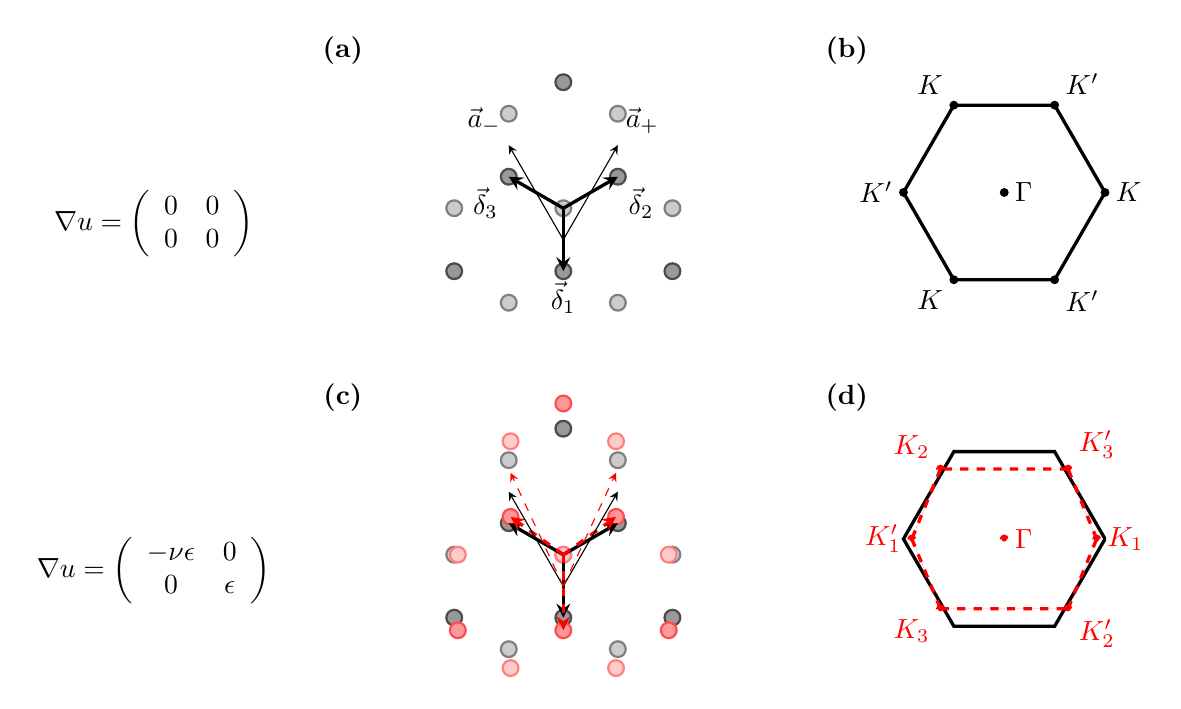
\begin{tikzpicture}[>=stealth,scale=.8,
		nnarrow/.style={color=black,very thick, ->},					% Nearest neighbor vectors
		nnarrows/.style={color=red,very thick, dashed, ->},				% Strained nearest neighbor vectors		
		lvarrow/.style={color=black, ->},								% lattice vector unstrained
		lvarrows/.style={color=red, dashed, ->},						% Lattice vector strained
		BZ/.style={color=black,fill=black,very thick},					% Unstrained BZ lines
		BZs/.style={color=red,fill=red,dashed, very thick},				% Strained BZ lines
		circ2/.style={radius=1.5pt},									% Dots at K points on BZ
		A/.style={circle,draw=black!50,fill=black!20,
			thick,minimum size=2 mm,inner sep=0pt}, 					% A sublattice dots (unstrained)
		As/.style={circle,draw=red!50,fill=red!20,
			thick,minimum size=2 mm,inner sep=0pt}, 					% A sublattice dots (strained)
		B/.style={circle,draw=black!70,fill=black!40,
			thick,minimum size=2mm,inner sep=0pt},						% B sublattice dots (strained)
		Bs/.style={circle,draw=red!70,fill=red!40,
			thick,minimum size=2mm,inner sep=0pt}]						% B sublattice dots (unstrained)					

	% Graphene lattice, sublattices different colors, nearest neighbor vectors and lattice vectors
	\begin{scope}[xshift=-3.5 cm,yshift=1.5 cm]				% Lattice vector arrows

		%This scope is clipped to limit the drawn lattice to a square
		\clip (-2.75cm,-2cm) rectangle(2.75cm,2.75cm);
		% \draw (-2.75cm,-2cm) rectangle(2.75cm,2.75cm);

		% Draw the unstrained lattice
		\foreach \ip in {-1,0,...,1}
			\foreach \im in {-1,0,...,1}
			{
			\node at (\ip*\sqth*\alat/2-\im*\sqth*\alat/2, \ip*\alat*3/2+\im*\alat*3/2      ) [A] {};
			\node at (\ip*\sqth*\alat/2-\im*\sqth*\alat/2, \ip*\alat*3/2+\im*\alat*3/2-\alat) [B] {};
			}

		% Draw the nearest neighbor vectors
		\draw[nnarrow] (0,0) -- +(270:\alat) node[anchor=north     ]{$\vec{\delta}_1$};
		\draw[nnarrow] (0,0) -- +( 30:\alat) node[anchor=north west]{$\vec{\delta}_2$};
		\draw[nnarrow] (0,0) -- +(150:\alat) node[anchor=north east]{$\vec{\delta}_3$};
		
		% Draw the lattice vectors
		\draw[lvarrow] (0,-\alat/2) -- +( 60:\sqth*\alat)node[circle,anchor=south west]{$\vec{a}_+$};
		\draw[lvarrow] (0,-\alat/2) -- +(120:\sqth*\alat)node[circle,anchor=south east]{$\vec{a}_-$};
	\end{scope}

	% Reciprocal space BZ and high symmetry points
	\begin{scope}[xshift=3.5cm,yshift=1.75 cm,scale=.8]

		% Draw the BZ
		\draw[BZ]
			(  0:\Klen) circle[circ2] node[anchor=west      ]{$\bm{K} $} --
			( 60:\Klen) circle[circ2] node[anchor=south west]{$\bm{K'}$} --
			(120:\Klen) circle[circ2] node[anchor=south east]{$\bm{K }$} -- 
			(180:\Klen) circle[circ2] node[anchor=east      ]{$\bm{K'}$} -- 
			(240:\Klen) circle[circ2] node[anchor=north east]{$\bm{K }$} -- 
			(300:\Klen) circle[circ2] node[anchor=north west]{$\bm{K'}$} -- 
			(  0:\Klen);

		% Label the high symmetry points
		\draw[BZ] (0,0) circle[circ2] node[anchor=west]{$\Gamma$};
	\end{scope}

	% Strained lattice
	\begin{scope}[xshift=-3.5 cm,yshift=-4 cm]
		%This scope is clipped to limit the drawn lattice to a square
		\clip (-2.75cm,-2cm) rectangle(2.75cm,2.75cm);
		% \draw (-2.75cm,-2cm) rectangle(2.75cm,2.75cm);

		% Draw the unstrained lattice
		\foreach \ip in {-1,0,...,1}
			\foreach \im in {-1,0,...,1}
			{
			\node at (\ip*\sqth*\alat/2-\im*\sqth*\alat/2, \ip*\alat*3/2+\im*\alat*3/2      ) [A] {};
			\node at (\ip*\sqth*\alat/2-\im*\sqth*\alat/2, \ip*\alat*3/2+\im*\alat*3/2-\alat) [B] {};
			}

		% Draw the strained lattice
		\foreach \ip in {-1,0,...,1}
			\foreach \im in {-1,0,...,1}
			{
			\node at (\ip*.837*\alat-\im*.837*\alat, \ip*\alat*1.8+\im*\alat*1.8          ) [As] {};
			\node at (\ip*.837*\alat-\im*.837*\alat, \ip*\alat*1.8+\im*\alat*1.8-1.2*\alat) [Bs] {};
			}

		% Draw the unstrained nearest neighbor vectors
		\draw[nnarrow] (0,0) -- +(270:\alat);
		\draw[nnarrow] (0,0) -- +(30 :\alat);
		\draw[nnarrow] (0,0) -- +(150:\alat);

		% Draw the strained nearest neighbor vectors
		\draw[nnarrows] (0,0) -- +(    0*\alat,-1.2*\alat);
		\draw[nnarrows] (0,0) -- +( .837*\alat, .60*\alat);
		\draw[nnarrows] (0,0) -- +(-.837*\alat, .60*\alat);

		% Draw the unstrained lattice vectors
		\draw[lvarrow] (0,-\alat/2) -- +( 60:\sqth*\alat);
		\draw[lvarrow] (0,-\alat/2) -- +(120:\sqth*\alat);

		% Draw the strained lattice vectors
		\draw[lvarrows] (0,-\alat/2) -- +( .837*\alat,1.8*\alat);
		\draw[lvarrows] (0,-\alat/2) -- +(-.837*\alat,1.8*\alat); 
	\end{scope}

	% Strained BZ
	\begin{scope}[xshift=3.5 cm,yshift=-3.75 cm,scale=.8]
		% Draw the unstrained BZ
		\draw[color=black,very thick]
			(  0:\Klen)  --
			( 60:\Klen)  --
			(120:\Klen)  -- 
			(180:\Klen)  -- 
			(240:\Klen)  -- 
			(300:\Klen)  -- 
			(  0:\Klen);

		% Draw the strained 
		\draw[BZs]
			( .917*\Klen, .000*\Klen) circle[circ2] node[anchor=west      ]{$\bm{K_1} $} --
			( .633*\Klen, .693*\Klen) circle[circ2] node[anchor=south west]{$\bm{K_3'}$} --
			(-.633*\Klen, .693*\Klen) circle[circ2] node[anchor=south east]{$\bm{K_2}$} -- 
			(-.917*\Klen, .000*\Klen) circle[circ2] node[anchor=east      ]{$\bm{K_1'}$} -- 
			(-.633*\Klen,-.693*\Klen) circle[circ2] node[anchor=north east]{$\bm{K_3}$} -- 
			( .633*\Klen,-.693*\Klen) circle[circ2] node[anchor=north west]{$\bm{K_2'}$} -- 
			( .917*\Klen, .000*\Klen);

		% Label the high symmetry points
		\draw[BZs] (0,0) circle[circ2] node[anchor=west]{$\Gamma$};
	\end{scope}


	% (a) (b) (c) and (d) labels
	\node at (-7cm,4cm)   {\textbf{(a)}};
	\node at ( 1cm,4cm)   {\textbf{(b)}};
	\node at (-7cm,-1.5cm){\textbf{(c)}};
	\node at ( 1cm,-1.5cm){\textbf{(d)}};

	% Strain labels on the right side
	\node at (-10cm, 1.25 cm) {$\bm{\nabla u}=\left(\begin{array}{cc} 0 & 0 \\ 0 & 0 \end{array}\right)$};
	\node at (-10cm,-4.25 cm) {$\bm{\nabla u}=\left(\begin{array}{cc} -\nu \epsilon & 0 \\ 0 & \epsilon \end{array}\right)$};
\end{tikzpicture}
  \caption{\label{fig:PVP:lattice} (a) Unstrained graphene's real space lattice with labeled nearest neighbor vectors ($\vec{\delta_i}$), labeled lattice vectors, $\vec{a}_+$ and  $\vec{a}_-$, and with light and dark dots representing the A and B sub-lattices, respectively. (b) The Brillouin zone of unstrained graphene with labeled high symmetry points. (c) The change in the real space lattice after the application 20 \% uniaxial strain in the $\hat{y}$ direction.  Red dots represent the position of the strained atoms and red dashed lines are the strained nearest neighbor and lattice vectors which are referred to as $\vec{\delta}_i'$ and $\vec{a}_i'$ respectively.  (d) The unstrained (black, solid) and strained (red, dashed) Brillouin zone, also for 20 \% armchair uniaxial strain, with the now inequivelent inequivalent Dirac points labeled.  $\bm{\nabla u}$ is the displacement gradient tensor detailing the distortion for each row.}
\end{figure}

Figure \ref{fig:PVP:lattice}(c) provides a qualitative geometric picture for how strain alters the unstrained nearest neighbor tight binding approach discussed in Chapter \ref{chap:TB}.
The method of calculating the distortion of the real and reciprocal space lattices is discussed in detail later in this chapter.
The noticeable geometric distortion of both the nearest neighbor vectors and the lattice vectors corresponds to two distinct changes in the tight binding prescription.
The anisotropic alteration of the nearest neighbor vectors modifies the distances between atoms introducing a bond-dependent nearest neighbor hoping amplitude into the unstrained real space Hamiltonian (Equation \ref{eq:TB:baseham}) \cite{Hasegawa2006}
\begin{equation}
  H=-\sum_{<i,j>} \left( t_{i,j} a_i^{\dagger} b_j + t_{j,i} b_j^{\dagger} a_i \right) \ ,
  \label{eq:PVP:RealSpace}
\end{equation}
where $t_{i,j}$ is the bond specific hoping energy.
The second, and oft neglected alteration is a result of the distortion of the lattice vectors.
Their alteration necessitates a change in the phase factors in the Fourier expansion of the creation and annihilation operators in Equation \ref{eq:TB:FT},
\begin{align}
  a_i^{\dagger}&=\frac{1}{\sqrt{N}}\sum_{\vec{k} } e^{ i \vec{k}  \cdot \vec{R}_i'} a_{\vec{k} }^{\dagger} \nonumber \\
  b_j          &=\frac{1}{\sqrt{N}}\sum_{\vec{k}'} e^{-i \vec{k}' \cdot \vec{R}_j'} b_{\vec{k}'} \ . \label{eq:PVP:FT} 
\end{align}
where $\vec{R}_i'$ and $\vec{R}_j'$ are the positions of the atoms in the strained A and B sub-lattices respectively.
They are not controllable independently in an actual physical system; the latter is a consequence of the former.
Past works have ignored the modification of the relative positions of the atoms.

A necessary and non-trivial first step toward including these modifications in the tight binding description is determining how the lattice vectors and nearest neighbor vectors are altered by strain.
This directly determines how the Fourier transforms in Equation \ref{eq:TB:FT} should be altered and is also useful for determining how the hopings in Equation \ref{eq:TB:baseham} are altered.
In general the strain is not uniform and the distortion of these vectors has a spatial dependence.
In continuum mechanics the elastic deformation field, $\vec{u}(\vec{r})$, which detail the shifts in position generated by  deformation is calculated based on macroscopic quantities.
Here we follow the Cauchy-Born rule which projects these macroscopic quantities onto the atomic lattice.
In this approximation, the position of the $i$-th atom in the deformed configuration, $\vec{R}'_i$, is given with reference to the undeformed one, $\vec{R}_i$, in terms of the deformation field
\begin{equation*}
  \vec{R}'_{i}=\vec{R}_{i}+\vec{u}(\vec{R_i}) \ .
\end{equation*}
Although it is feasible that at the atomic scale the A and B sublattices behave differently yet still yield the same macroscopic response, the Cauchy-Born rule provides a simple and reasonable starting point for the discussion of strain effects.
The strained lattice vector at the $i$-th lattice site, $\vec{a}'_{i,\pm}$, is then given approximately by
\begin{align}
  \vec{a}'_{i,\pm}(\vec{r})&=\vec{R}'_j-\vec{R}'_i \nonumber\\
                              &=(\vec{R}_j-\vec{R}_i)+\vec{u}(\vec{R_j})-\vec{u}(\vec{R_i}) \nonumber \\
                              &\simeq\vec{a}_{i,\pm}+(\vec{a}_{i,\pm} \cdot \vec{\nabla}) \vec{u}(\vec{R}_i) \nonumber \\
                              &=\left(\bm{1}+\bm{\nabla u}(\vec{R_i}) \right)\cdot \vec{a}_{i,\pm} \label{eq:PVP:StrainVectors} \ ,
\end{align}
where $\bm{1}$ is the two dimensional identity matrix and the dyadic product $\bm{\nabla u}(\vec{R_i})$ is the Jacobian of the displacement field known as the displacement gradient tensor
\begin{align*}
  [\bm{\nabla u}]_{ij} = u_{i,j} &= \frac{u_{i,j}+u_{j,i}}{2} + \frac{u_{i,j}-u_{j,i}}{2} \\
                       &\equiv \tilde{\epsilon}_{ij} + \tilde{\omega}_{ij} \\
    \rightarrow \quad \bm{\nabla u} &= \tilde{\bm{\epsilon}} + \tilde{\bm{\omega}}
\end{align*}
where $\tilde{\bm{\omega}}$ is the rotation tensor and $\tilde{\bm{\epsilon}}$ is the \emph{linear} strain tensor which is only one part of the full (Lagrange) strain tensor given by $\bm{\epsilon} = \tfrac{1}{2}(\bm{\nabla u} + \bm{\nabla u}^\top+\bm{\nabla u}^\top\bm{\nabla u}) = \tilde{\bm{\epsilon}} + \tfrac{1}{2}(\bm{\nabla u}^\top\bm{\nabla u})$.
It is important to stress that the often used approximating $\vec{a}'_{i,\pm}(\bm{r})\simeq (\bm{1}+\tilde{\bm{\epsilon}})\cdot \vec{a}'_{i,\pm}$ is only valid if the deformation does not involve local rotation ($\tilde{\bm{\omega}}=0$).
To simplify the notation, the position dependence has been left off of $\bm{\nabla u}$.
Similarly, the strain modified nearest neighbor vectors are $\vec{\delta}'_{i,j}(\vec{r})=(\bm{1}+\bm{\nabla u}) \cdot \vec{\delta}_{j}(\vec{r})$ \cite{Kitt2013} where $i$ keeps track of the spatial dependence by indicating the unit cell and $j \in {1,2,3}$ indicates which of the three nearest neighbor vectors is being referred to.

The distortion of the nearest neighbor vectors causes a bond specific alteration of the hoping energy.
By comparing a tight binding treatment of strained graphene to density functional calculations of the same system, Ribeiro and coworkers showed that the dependence of the hoping energy on the distance between carbon atoms can be parameterized as:
\begin{equation*}
  t(|\vec{\delta}_{i,j}|)=t_0 \exp[-\beta (|\vec{\delta}_{i,j}|/a-1)]
\end{equation*}
with $\beta\approx 3$ \cite{Pereira2009,Ribeiro2009,CastroNeto2009}.
An exponential decay is chosen because it correctly predicts both the nearest neighbor and next nearest neighbor hoping energies.
The fact that, the hoping energy is mostly insensitive to the bond angle, greatly simplifies the physics.
Having already established the form for the strained nearest neighbor vectors, their length can be easily computed:
\begin{align*}
  |\delta'_{i,j}|^2&=\left(\vec{\delta}_{j}^{\intercal}+\vec{\delta}_{j}^{\intercal} \ \bf{\nabla u}^{\intercal} \right) \cdot
    \left(\vec{\delta}_{j}+\bf{\nabla u} \ \vec{\delta}_{j} \right) \\
    &=\vec{\delta}_{j}^{\intercal} \vec{\delta}_{j}+
      \vec{\delta}_{j}^{\intercal} \left(\bf{\nabla u}+\bf{\nabla u}^{\intercal} \right) \vec{\delta}_{j}+
      \mathcal{O}(\bf{\nabla u}^2) \\
  \rightarrow |\delta'_{i,j}|&\simeq a+\frac{1}{a} \vec{\delta}_{j} \cdot \tilde{\bm{\epsilon}} \cdot \vec{\delta}_{j}
\end{align*}
for small strains.
As was done for the displacement gradient tensor, the spatial dependence of the strain tensor is dropped from the notation for simplicity.
As expected, the length of these vectors are dependent only on the symmetric part of the displacement gradient tensor-the strain.
To first order, the bond specific nearest neighbor hoping can be written as
\begin{equation*}
  t_{i,j}=t_0+\delta t_{i,j}=t_0-\beta t_0 \frac{1}{a^2} \vec{\delta}_{j} \cdot \tilde{\bm{\epsilon}} \cdot \vec{\delta}_{j},
\end{equation*}
or
\begin{align}
  \delta t_{i,1}&=-\beta t_0 \tilde{\epsilon}_{yy} \nonumber \\
  \delta t_{i,2}&=-\beta t_0 \left( \frac{3}{4}\tilde{\epsilon}_{xx} +\frac{1}{4} \tilde{\epsilon}_{yy} + \frac{\sqrt{3}}{2} \tilde{\epsilon}_{xy} \right) \nonumber \\
  \delta t_{i,3}&=-\beta t_0 \left( \frac{3}{4}\tilde{\epsilon}_{xx} +\frac{1}{4} \tilde{\epsilon}_{yy} - \frac{\sqrt{3}}{2} \tilde{\epsilon}_{xy} \right)  \label{eq:PVP:dtij}\ .
\end{align}
This fully defines the strain dependences of the modifications in Equations \ref{eq:PVP:RealSpace} and \ref{eq:PVP:FT}.

All the pieces necessary to modify the nearest neighbor tight binding approach from Chapter \ref{chap:TB} are now in place.
The first modification to include the approximated hoping energy in Equation \ref{eq:PVP:RealSpace},
\begin{equation*}
  H=-\sum_{<i,j>} \left( (t_0+\delta t_{i,j})  a_i^{\dagger} b_j + (t_0+\delta t_{j,i}) b_j^{\dagger} a_i \right) \ .
\end{equation*}
In situations such as the deformation of graphene around a sharp scanning tunneling microscopy tip, is not necessarily true that $\delta t_{i,j} = \delta t_{j,i}$.
In these extreme strain situations the continuum approximation can breaks down, the sub-lattice symmetry can be broken, and it is possible that $\delta t_{i,j} \neq \delta t_{j,i}$.
However, for strains that vary slowly with respect to the lattice spacing, the continuum approximation hold and $\delta t_{i,j} \simeq \delta t_{j,i}$ \cite{Sloan2013}.
This assumption will be made throughout.
As a result, the real space Hamiltonian in Equation \ref{eq:PVP:RealSpace} can be approximated to first order in strain,
\begin{equation*}
  H \simeq -\sum_{<i,j>} \left( t_0+\delta t_{i,j} \right)  a_i^{\dagger} b_j + \text{H.C.} \ ,
\end{equation*}
with the strain dependence of $\delta t_{i,j}$ given by Equation \ref{eq:PVP:FT}.

Using the Fourier transforms of the creation and annihilation operators in Equation \ref{eq:PVP:FT}, the Hamiltonian is written in reciprocal space as 
\begin{equation*}
  H=-\frac{1}{N} \sum_{<i,j>} \sum_{\vec{k},\vec{k}'} \left( t_0+\delta t_{i,j} \right)
    e^{i(\vec{k}-\vec{k}')\cdot \vec{R}_i'}
    e^{-i\vec{k}'\cdot \vec{\Delta}_{i,j}'}
    a_{\vec{k}}^{\dagger} b_{\vec{k'}} +\text{H.C.}\ ,
\end{equation*}
where $\vec{\Delta}_{i,j}=\vec{R}_j'-\vec{R}_i'$.
As compared to the unstrained case in Equation \ref{eq:TB:FTing}, the $i$ dependence is not isolated to a single term.
Instead, the strain can vary throughout the lattice resulting in the $i$ dependence of $\vec{\Delta}_{i,j}$.
%----Justify why we drop the $i$ dependence here to define slowly varying.

When isolated, the remaining $i$ dependence corresponds to a Fourier Transform of the hoping energy,
\begin{align*}
  \tilde{t}_{\vec{k}-\vec{k}'}&=\sum_i \left( t_0+\delta t_{i,j} \right) e^{i(\vec{k}-\vec{k}')\cdot \vec{R}_i'} \\
                              &=N t_0 \delta_{\vec{k},\vec{k}'}+\sum_i \delta t_{i,j} e^{i(\vec{k}-\vec{k}')\cdot \vec{R}_i'} \ .
\end{align*}
Only specific Fourier components yield relevant $\tilde{t}_{\vec{k}-\vec{k}'}$ when working in the low energy regime.
The wave-vectors will again be approximated as $\vec{k}=\bm{K}+\vec{q}$ and $\vec{k}=\bm{K'}+\vec{q}$ for small $qa$, giving
\begin{align*}
  \tilde{t}_{\vec{k}-\vec{k}'}&\simeq N t_0 \delta_{\vec{k},\vec{k}'} + 
    \sum_i \delta t_{i,j} e^{i(\bm{K^{(')}}+\vec{q}-\bm{K^{(')}}-\vec{q}') \cdot \vec{R}_i'} \\
                              &\simeq N t_0 \delta_{\vec{k},\vec{k}'} + 
    \sum_i \delta t_{i,j} e^{i(\bm{K^{(')}}-\bm{K^{(')}}) \cdot \vec{R}_i'} (1+(\vec{q}-\vec{q}') \cdot \vec{R}_i') \\
                              &\simeq N t_0 \delta_{\vec{k},\vec{k}'} + 
    \sum_i \delta t_{i,j} e^{i(\bm{K^{(')}}-\bm{K^{(')}}) \cdot \vec{R}_i'} \ ,
\end{align*}
where $\bm{K^{(')}}$ refers to either $\bm{K}$ or $\bm{K'}$ depending on the wave-vector.
Thus, to first order in the small parameters the only relevant Fourier components are for $\vec{k}-\vec{k}' \in \{0,\bm{K}-\bm{K'}, \bm{K'}-\bm{K} \}$.
The high frequency components could interestingly act to couple the $\bm{K}$ and $\bm{K}'$ points.
However, since the strain is assumed to be slowly varying here, we eliminate the high frequency components and limit $\vec{k}-\vec{k}' \rightarrow 0$, yielding
\begin{equation*}
  \tilde{t}_{\vec{k}-\vec{k}'}\simeq N \delta_{\vec{k},\vec{k}'} (t_0 + <\delta t_{i,j}>) \ .
\end{equation*}
where $<\delta t_{i,j}>$ is the average value over $i$ of $\delta t_{i,j}$ which will be written as $\delta t_j$.

The Hamiltonian is now simplified to
\begin{equation*}
    H=-\sum_{\vec{k}} \sum_{j} \left( t_0+\delta t_j \right)
    e^{-i\vec{k}'\cdot \vec{\Delta}_{i,j}'}
    a_{\vec{k}}^{\dagger} b_{\vec{k}} +\text{H.C.} \ .
\end{equation*}
By applying the low energy approximation as well as using the form for the strained vectors in Equation \ref{eq:PVP:StrainVectors}, the Hamiltonian can be approximated in terms of the three small parameters: $qa$, $\tilde{\bm{\epsilon}}$, $\bm{\nabla u}$.
Near $\bm{K}$ the Hamiltonian becomes 
\begin{align*}
  H\simeq& -\sum_{\vec{q}} \sum_{j} \left( t_0+\delta t_j \right)
    e^{-i (\bm{K}+\vec{q}) \cdot (\bm{1}+\bm{\nabla u}) \cdot \vec{\Delta}_{j}}
    a_{\vec{k}}^{\dagger} b_{\vec{k}} +\text{H.C.} \\
   \simeq& -\sum_{\vec{q}} \sum_{j} \left( t_0+\delta t_j \right) e^{-i \bm{K} \cdot \vec{\Delta}_j}
    (1-i \vec{q} \cdot \vec{\Delta_j}) (1-i\bm{K}\cdot \bm{\nabla u} \cdot \vec{\Delta}_j)
    a_{\vec{k}}^{\dagger} b_{\vec{k}} +\text{H.C.} \\
   \simeq& 
    -t_0 \sum_{\vec{q}} \sum_{j} (1-i\vec{q} \cdot \vec{\Delta_j}) e^{-i \bm{K} \cdot \vec{\Delta}_j} a_{\vec{k}}^{\dagger}b_{\vec{k}}
    -\sum_{\vec{q}} \sum_{j} \delta t_j e^{-i \bm{K} \cdot \vec{\Delta}_j} a_{\vec{k}}^{\dagger}b_{\vec{k}} \\
    &+i t_0 \bm{K} \cdot \bm{\nabla u} \sum_{\vec{q}} \cdot \sum_{j} \vec{\Delta}_j e^{-i \bm{K} \cdot \vec{\Delta}_j} a_{\vec{k}}^{\dagger}b_{\vec{k}}
    +\text{H.C.} \\
   =& H_0+H_{hoping}+H_{lattice}
\end{align*}
with a similar form near $\bm{K'}$ except with $\bm{K}$ replaced with $\bm{K'}$.
The full Hamiltonian nicely breaks up into three parts.
The first part, $H_0=-t_0 \sum_{\vec{q}} \sum_{j} (1-i\vec{q} \cdot \vec{\Delta_j}) e^{-i \bm{K} \cdot \vec{\Delta}_j} a_{\vec{k}}^{\dagger}b_{\vec{k}}+\text{H.C.}$, exactly matches the low energy Hamiltonian of unstrained graphene from Equations \ref{eq:TB:LowEnergy} and \ref{eq:TB:FTing}.
Strain, then, acts to perturb the unstrained Hamiltonian through $H_{hoping}=-\sum_{\vec{q}} \sum_{j} \delta t_j e^{-i \bm{K} \cdot \vec{\Delta}_j} a_{\vec{k}}^{\dagger}b_{\vec{k}}+\text{H.C.}$ and $H_{lattice}=i t_0 \bm{K} \cdot \bm{\nabla u} \sum_{\vec{q}} \cdot \sum_{j} \vec{\Delta}_j e^{-i \bm{K} \cdot \vec{\Delta}_j} a_{\vec{k}}^{\dagger}b_{\vec{k}}+\text{H.C.}$.
Geometrically, the first term originates from the deformation of the nearest neighbor vectors, shown in Figure \ref{fig:PVP:lattice}, which causes the bond specific hoping energy.
The second term corresponds to the deformation of the lattice vectors, also shown in Figure \ref{fig:PVP:lattice}.
Before it was originally introduced by Kitt et al \cite{Kitt2012}, the second term was neglected.
The lattice was treated as if it were undeformed and strain only acted to alter the interactions between nearest neighbors.
However, both of the perturbations are first order in small parameters; $H_{hoping}$ is $\mathcal{O}(\tilde{\bm{\epsilon}})$ while $H_{lattice}$ is $\mathcal{O}(\bm{\nabla u})$.
Consequently, they contributes on equal footing and $H_{lattice}$ should be included.

The perturbations $H_{hopping}$ and $H_{lattice}$ mimic the effects of a magnetic field.
In the minimum coupling scenario the presence of a magnetic field is accounted through the substitution $\vec{p} \rightarrow \vec{p} - e \vec{A}$ where $A$ is the vector potential which is related to the magnetic field through $\vec{B}=\nabla \times \vec{A}$.
The perturbations $H_{hoping}$ and $H_{lattice}$ contribute a similar shift in the crystal momentum $\vec{\hbar k} \rightarrow \vec{\hbar k} - e \vec{\mathcal{A}}$ where $\vec{\mathcal{A}}$ is the pseudo vector potential.
This formalism uses the \emph{undeformed} BZ as global reference to which the strain induced shifts of the momentum are measured.
This identification can be made because the perturbations contribute to the same matrix elements as $H_0$: they are off diagonal and do not couple the $\bm{K}$ and $\bm{K'}$ points.
Further, they provide only a strain dependent complex offset independent of the crystal momentum.
The form of $H_0$ shown in Equation \ref{eq:TB:FullH} allows the isolation of the x and y components of $\vec{\mathcal{A}}$ from the real and imaginary parts of the perturbations as
\begin{align*}
  \mathcal{A}_{x,\bm{K}}&=-\vec{\mathcal{A}}_{x,\bm{K'}}=-\frac{1}{v_f e} Re[h_{hoping}+h_{lattice}] \\
  \mathcal{A}_{y,\bm{K}}&=\vec{\mathcal{A}}_{y,\bm{K'}}= \frac{1}{v_f e} Im[h_{hoping}+h_{lattice}] \ ,
\end{align*}
where $h_{hopping}=-\sum_{j} \delta t_j e^{-i \bm{K} \cdot \vec{\Delta}_j}$ and $h_{lattice}=i t_0 \bm{K} \cdot \bm{\nabla u} \cdot \sum_{j} \vec{\Delta}_j e^{-i \bm{K} \cdot \vec{\Delta}_j}$.
The resulting pseudo vector potentials are:
\begin{align}
  \vec{\mathcal{A}}_{\bm{K_1}}&=-\vec{\mathcal{A}}_{\bm{K_1'}}=
    \frac{\phi_0}{2a} \left( \begin{array}{c} 
      -\frac{4}{3\sqrt{3}} [\bm{\nabla u}]_{xx} \\ 
      -\frac{4}{3\sqrt{3}} [\bm{\nabla u}]_{xy}
    \end{array} \right) +\vec{A}_p \nonumber \\ 
  \vec{\mathcal{A}}_{\bm{K_2}}&=-\vec{\mathcal{A}}_{\bm{K_2'}}=
    \frac{\phi_0}{2a} \left( \begin{array}{c} 
      \frac{2}{3\sqrt{3}}[\bm{\nabla u}]_{xx}-\frac{2}{3} [\bm{\nabla u}]_{yx} \\
      -\frac{2}{3} [\bm{\nabla u}]_{yy}+\frac{2}{3 \sqrt{3}} [\bm{\nabla u}]_{xy}
    \end{array} \right)+\vec{A}_p  \nonumber \\
  \vec{\mathcal{A}}_{\bm{K_3}}&=-\vec{\mathcal{A}}_{\bm{K_3'}}=
    \frac{\phi_0}{2a} \left( \begin{array}{c}
      \frac{2}{3\sqrt{3}}[\bm{\nabla u}]_{xx}+\frac{2}{3} [\bm{\nabla u}]_{yx} \\
      \frac{2}{3} [\bm{\nabla u}]_{yy}+\frac{2}{3 \sqrt{3}} [\bm{\nabla u}]_{xy}
    \end{array} \right)+\vec{A}_p  , \nonumber \\
  \textrm{with }
  &\vec{\mathcal{A}}_p= 
    \frac{\phi_0}{2a} \left( \begin{array}{c} 
      \frac{\beta }{2 \pi} (\tilde{\epsilon}_{xx}-\tilde{\epsilon}_{yy}) \\
      -\frac{\beta}{\pi} \tilde{\epsilon}_{xy}
    \end{array} \right),
  \label{eq:PVP:PVP}
\end{align}
$\phi_0=\frac{h}{e}$, and the various $\bm{K}_i$ points are defined as in Figure \ref{fig:PVP:lattice}(d).
The common term $\vec{\mathcal{A}}_p$ is proportional to the logarithmic derivative of the hoping, $\beta$, and arises from the hoping perturbations, $\delta t_j$, alone.
It has the expected dependence on the strain tensor components \cite{CastroNeto2009,Vozmediano2010}. 
The herein derived additional terms are the corrections due to lattice deformations.
Since $\beta \approx 3$, the lattice corrections are equally important, not only for being of the same order in strain, but for having similar numerical coefficients.
It is also worth emphasizing that taking explicit consideration of the lattice deformations leads to a vector potential that is different for all the corners of the BZ.
This is of course expected because under an arbitrary deformation the equivalence among the three $\bm{K}$ and $\bm{K'}$ points is lost.
In fact, the expressions above quantify the fact that upon general deformation of the graphene lattice, the Dirac point no longer lies at $\bm{K_i}$, nor at any of the symmetry points of the deformed BZ, a point emphasized early on \cite{Pereira2009}.
The only remaining constraint is time-reversal symmetry, which forces $\vec{\mathcal{A}}_{\bm{K_i}} = - \vec{\mathcal{A}}_{\bm{K_i'}}$.
In contrast to a real vector potential, strain generated pseudo vector potentials can not break time reversal symmetry.

It should be noted that the pseudovector potential depends on the crystallographic orientation relative to the strain.
Uniaxial strain of the same macroscopic value but at a different crystallographic orientation will result in different pseudo vector potentials.
The form for the pseudo vector potential assume that the tensors are written such that the x axis is aligned with a zig zag direction.
They can be rewritten for different orientations by rotating the tensors so that their x axis is aligned with the zig zag direction, calculating the pseudo vector potential using Equations \ref{eq:PVP:PVP}, and then rotate the resulting pseudo vector potential back into the original reference frame.

\begin{figure*}
\includegraphics{Figs_PVP/figure_2.pdf}
\caption{(Color online) Contours of the band structure of graphene under tensile isotropic strain, shear strain, uniaxial armchair strain, and zig-zag strain (rows), for $\epsilon=1\%$ near the three $\bm{K}$ points (columns). The contours are overlaid with the Brillouin zone of unstrained (solid, black)  and strained (dashed, brown) graphene. Vectors mark the displacement of the Dirac points predicted by the traditional ($\vec{A}_p$, dashed/red arrow) and the corrected ($\vec{A}_{\bm{K}_{\!i}}$, solid/orange arrow) form of the pseudo vector potential (eqs.~\ref{pvp-all}), with the green dots marking the positions of the Dirac points for strained graphene. The red vectors appears as a dot for isotropic strain because the traditional form of the vector potential does not predict a shift in the Dirac points.  Each plot is square with an area of $0.12^2$. \label{fig:PVP:PVPshifts}}
\end{figure*}


\section{Discussion}

All existing calculations consider only the term $\vec{A}_p$ and, as a result do not properly account for the shift in the Dirac points.
Consider, for example, the seemingly trivial case of tensile isotropic strain.
The traditional form of the pseudovector potential, $\vec{A}_p$, predicts that there should be no shift in the Dirac points ($\epsilon_{xx}=\epsilon_{yy}$ and $\epsilon_{xy}=0$ in equation \ref{pvpe}).
However, the BZ shrinks isotropically under tensile isotropic strain, and, by symmetry, the Dirac points should follow the corners of the deformed BZ resulting in a Dirac point dependent shift toward the $\Gamma$ point with respect to the unstrained reference state.
In Fig.~\ref{PVPshifts}, the reciprocal space shifts of the Dirac points predicted by the traditional and herein corrected forms of the pseudovector potential are compared.
The contours are the strained band structure calculated using a nearest neighbor tight binding model which accounts for both the strain induced changes in hoping amplitudes and the lattice deformation \cite{Pereira2009}.
For isotropic tensile strain, the lattice-corrected pseudo vector potential in eqs.~\eqref{pvp-all} properly predicts the displacement of each Dirac point due to strain.
The less trivial cases of uniaxial or shear strain are also shown in Fig.~\ref{PVPshifts}. The differences between the red (traditional) and orange (corrected) arrows make it clear that the lattice corrections are needed to determine the absolute position of the Dirac point in reciprocal space (they can even reverse the sign of $\vec{A}$).

As discussed above, these corrections are immaterial for systems with spatially uniform strain but must be included for systems with non-uniform strain.
For example, if there are regions of isotropic tension embedded in regions of different strain states, the relative shifts \emph{are} important, even though deformations are locally isotropic.
In these cases lattice corrections contribute an extra, Dirac point specific, space dependence which is important when calculating transport across a strain barrier or when considering the spatial distribution of the pseudomagnetic fields: $\vec{B}_{\bm{K_i}} = \nabla \times \vec{A}_{\bm{K_i}}$.

In particular, these corrections are critical when trying to optimize the Landau quantization caused by the strain-induced pseudomagnetic fields.
Ideally one desires the pseudomagnetic field to be nearly constant throughout the system so that the Landau levels are as narrow and well defined as possible.
This imposes a delicate and non-trivial constraint on what deformations are compatible with constant pseudomagnetic fields.
An early suggestion uses the traditional form of the pseudovector potential to conclude that strain profiles with an overall trigonal symmetry tend to generate smooth effective pseudomagnetic fields \cite{Guinea2009}.
To show how the lattice correction can quantitatively and qualitatively affect this conclusion, we simulate a situation where graphene is covering an equilateral triangular pit with a uniformly distributed vertical load.
This geometry was originally proposed by Guinea~\emph{et~al.} as a simple method of generating fairly uniform pseudomagnetic fields \cite{Guinea2009}.
We calculate the strain fields using finite element analysis, and extract the local pseudomagnetic fields from eqs.~\eqref{pvp-all}.
The finite element analysis was performed using Comsol Multiphysics, with a two-dimensional thin plate model including geometric non-linearity.
The edges were fixed and the pressure was applied using a face load.
Graphene's Young's Modulus of 1 TPa and thickness of 3.5 \AA \cite{Lee2008} were used along with the Poisson ratio of graphite of 0.165 \cite{Blakslee1970}.
To make the triangles more realistic we include 2 nm radius fillets on the three corners, which smooth down the sharp boundary corners.
The surface was meshed with triangles with a maximum element size of 1 nm, and strain fields were evaluated in the mid-plane of the plate.

The second subtle point is that the pseudo vector potential has no gauge freedom.
Although it is true that there are a range of 

\begin{figure*}
\includegraphics{Figs_PVP/figure_3.pdf}
\caption{\label{triholes}The spatial distribution of the pseudomagnetic fields generated when an equilateral triangle with 50 nm sides, 2 nm radius fillets, and the base oriented 30 degrees counterclockwise from the armchair direction is pressurized to 14 MPa. In (a) the calculation is done using the traditional form of the pseudovector potential, while in (b) it is performed including the corrections derived in this work. Here, the three different colored curves correspond to the pseudomagnetic fields felt by the electrons at the three different $\bm{K}$ points with the magnetic field for the electrons at $\bm{K_1}$ isolated in (c). (Color online)}
\end{figure*}

The effect of the lattice corrections to the extracted pseudomagnetic field are shown in Fig.~\ref{triholes} for an equilateral triangle with 50 nm sides, and under 14 MPa of pressure.
At this pressure the graphene sheet has less than 0.26~\% strain.
The field derived from the traditional form of the pseudovector potential \eqref{pvpe} results in a fairly uniform pseudomagnetic field [Fig.~\ref{triholes}(a)], in agreement with Guinea et al \cite{Guinea2009}.
In contrast, Figs.~\ref{triholes}(b,c) show that the new terms cause the electrons near the three different $\bm{K}_{1,2,3}$ points to experience different pseudomagnetic fields, which vary strongly across the system.
The differences in the pseudomagnetic fields at the different Dirac points may be extremely useful in the context of valleytronics \cite{Rycerz2007}.

\section{Conclusion}

In summary, accounting for explicit lattice deformations in the calculation of the pseudo vector potentials generates new leading order, and $\bm{K}$ point specific terms, that are needed to accurately describe the strain dependent shift of the Dirac points in reciprocal space. These terms are important in situations of non-uniform strain, such as when exploring transmission across strain barriers, or when predicting pseudomagnetic fields arising from particular strain profiles.
In those situations the precise space dependence of the pseudo vector potentials, $\vec{A}_{\bm{K}_i}$, and the understanding that they are different at each of the three inequivalent Dirac points is important.

\setlength{\parindent}{0em}
\setlength{\parskip}{1em}

%__________________________________________________________________________________________________________________


The second conclusion is incorrect because, although the corrections $\vec{A}_\text{latt}$ are finite and, in general, have a position dependence, their rotational is identically zero and, thus, so is their contribution to the pseudomagnetic field. This has been pointed out recently by de Juan \emph{et al.}~\cite{DeJuan2013}. Below we elaborate on that, and on the reason why Fig.~3 apparently shows a non-zero $\vec{B}_{\bm{K}_i}$, when it should have been zero by construction. We trust the detail will benefit the reader.




When the correct expansion for the strained position of the atoms is used, it becomes apparent that the lattice corrections cannot contribute to the pseudomagnetic field. Upon expansion around a corner of the BZ of the undeformed lattice, $\bm{K}$, the lattice corrections to the vector potential can be cast as \cite{DeJuan2013}
%
\begin{equation}
  \vec{A}_\text{latt}=\vec{A}_{\bm{K}}-\vec{A}_p \propto \bm{\nabla} (\bm{K}\cdot\bm{u})
  .
\end{equation}
%
Since the above is a total derivative, it cannot contribute to the pseudomagnetic field because $\nabla\times\nabla \phi \equiv 0$. This can be also verified by direct inspection of Eqs.~(4) of the original paper which remain valid in form if the replacement $\bm{\epsilon } \to \bm{ \nabla u }$ is made.

Having clarified and established the correct expansion of the nearest neighbor vector and the lack of an induced pseudomagnetic field a few comments on the results in the original paper are in order:
%
\begin{enumerate} \renewcommand{\theenumi}{\roman{enumi}}
  \item The lattice corrections are still needed to correctly describe the shift in the positions of the Dirac points due to strain. Thus, when the position of the Dirac points is required in a global frame of reference (e.g. to describe momentum-sensitive electronic tunneling to/from strained graphene from/to another system, probe, or contact), Eqs.~4 should be used with the substitution $\bm{\epsilon } \to \bm{\nabla u}$:

\end{enumerate}